\documentclass[]{book}
\usepackage{lmodern}
\usepackage{amssymb,amsmath}
\usepackage{ifxetex,ifluatex}
\usepackage{fixltx2e} % provides \textsubscript
\ifnum 0\ifxetex 1\fi\ifluatex 1\fi=0 % if pdftex
  \usepackage[T1]{fontenc}
  \usepackage[utf8]{inputenc}
\else % if luatex or xelatex
  \ifxetex
    \usepackage{mathspec}
  \else
    \usepackage{fontspec}
  \fi
  \defaultfontfeatures{Ligatures=TeX,Scale=MatchLowercase}
\fi
% use upquote if available, for straight quotes in verbatim environments
\IfFileExists{upquote.sty}{\usepackage{upquote}}{}
% use microtype if available
\IfFileExists{microtype.sty}{%
\usepackage{microtype}
\UseMicrotypeSet[protrusion]{basicmath} % disable protrusion for tt fonts
}{}
\usepackage[margin=1in]{geometry}
\usepackage{hyperref}
\hypersetup{unicode=true,
            pdftitle={Reporting with Data in R},
            pdfauthor={Christian McDonald},
            pdfborder={0 0 0},
            breaklinks=true}
\urlstyle{same}  % don't use monospace font for urls
\usepackage{natbib}
\bibliographystyle{apalike}
\usepackage{color}
\usepackage{fancyvrb}
\newcommand{\VerbBar}{|}
\newcommand{\VERB}{\Verb[commandchars=\\\{\}]}
\DefineVerbatimEnvironment{Highlighting}{Verbatim}{commandchars=\\\{\}}
% Add ',fontsize=\small' for more characters per line
\usepackage{framed}
\definecolor{shadecolor}{RGB}{248,248,248}
\newenvironment{Shaded}{\begin{snugshade}}{\end{snugshade}}
\newcommand{\KeywordTok}[1]{\textcolor[rgb]{0.13,0.29,0.53}{\textbf{#1}}}
\newcommand{\DataTypeTok}[1]{\textcolor[rgb]{0.13,0.29,0.53}{#1}}
\newcommand{\DecValTok}[1]{\textcolor[rgb]{0.00,0.00,0.81}{#1}}
\newcommand{\BaseNTok}[1]{\textcolor[rgb]{0.00,0.00,0.81}{#1}}
\newcommand{\FloatTok}[1]{\textcolor[rgb]{0.00,0.00,0.81}{#1}}
\newcommand{\ConstantTok}[1]{\textcolor[rgb]{0.00,0.00,0.00}{#1}}
\newcommand{\CharTok}[1]{\textcolor[rgb]{0.31,0.60,0.02}{#1}}
\newcommand{\SpecialCharTok}[1]{\textcolor[rgb]{0.00,0.00,0.00}{#1}}
\newcommand{\StringTok}[1]{\textcolor[rgb]{0.31,0.60,0.02}{#1}}
\newcommand{\VerbatimStringTok}[1]{\textcolor[rgb]{0.31,0.60,0.02}{#1}}
\newcommand{\SpecialStringTok}[1]{\textcolor[rgb]{0.31,0.60,0.02}{#1}}
\newcommand{\ImportTok}[1]{#1}
\newcommand{\CommentTok}[1]{\textcolor[rgb]{0.56,0.35,0.01}{\textit{#1}}}
\newcommand{\DocumentationTok}[1]{\textcolor[rgb]{0.56,0.35,0.01}{\textbf{\textit{#1}}}}
\newcommand{\AnnotationTok}[1]{\textcolor[rgb]{0.56,0.35,0.01}{\textbf{\textit{#1}}}}
\newcommand{\CommentVarTok}[1]{\textcolor[rgb]{0.56,0.35,0.01}{\textbf{\textit{#1}}}}
\newcommand{\OtherTok}[1]{\textcolor[rgb]{0.56,0.35,0.01}{#1}}
\newcommand{\FunctionTok}[1]{\textcolor[rgb]{0.00,0.00,0.00}{#1}}
\newcommand{\VariableTok}[1]{\textcolor[rgb]{0.00,0.00,0.00}{#1}}
\newcommand{\ControlFlowTok}[1]{\textcolor[rgb]{0.13,0.29,0.53}{\textbf{#1}}}
\newcommand{\OperatorTok}[1]{\textcolor[rgb]{0.81,0.36,0.00}{\textbf{#1}}}
\newcommand{\BuiltInTok}[1]{#1}
\newcommand{\ExtensionTok}[1]{#1}
\newcommand{\PreprocessorTok}[1]{\textcolor[rgb]{0.56,0.35,0.01}{\textit{#1}}}
\newcommand{\AttributeTok}[1]{\textcolor[rgb]{0.77,0.63,0.00}{#1}}
\newcommand{\RegionMarkerTok}[1]{#1}
\newcommand{\InformationTok}[1]{\textcolor[rgb]{0.56,0.35,0.01}{\textbf{\textit{#1}}}}
\newcommand{\WarningTok}[1]{\textcolor[rgb]{0.56,0.35,0.01}{\textbf{\textit{#1}}}}
\newcommand{\AlertTok}[1]{\textcolor[rgb]{0.94,0.16,0.16}{#1}}
\newcommand{\ErrorTok}[1]{\textcolor[rgb]{0.64,0.00,0.00}{\textbf{#1}}}
\newcommand{\NormalTok}[1]{#1}
\usepackage{longtable,booktabs}
\usepackage{graphicx,grffile}
\makeatletter
\def\maxwidth{\ifdim\Gin@nat@width>\linewidth\linewidth\else\Gin@nat@width\fi}
\def\maxheight{\ifdim\Gin@nat@height>\textheight\textheight\else\Gin@nat@height\fi}
\makeatother
% Scale images if necessary, so that they will not overflow the page
% margins by default, and it is still possible to overwrite the defaults
% using explicit options in \includegraphics[width, height, ...]{}
\setkeys{Gin}{width=\maxwidth,height=\maxheight,keepaspectratio}
\IfFileExists{parskip.sty}{%
\usepackage{parskip}
}{% else
\setlength{\parindent}{0pt}
\setlength{\parskip}{6pt plus 2pt minus 1pt}
}
\setlength{\emergencystretch}{3em}  % prevent overfull lines
\providecommand{\tightlist}{%
  \setlength{\itemsep}{0pt}\setlength{\parskip}{0pt}}
\setcounter{secnumdepth}{5}
% Redefines (sub)paragraphs to behave more like sections
\ifx\paragraph\undefined\else
\let\oldparagraph\paragraph
\renewcommand{\paragraph}[1]{\oldparagraph{#1}\mbox{}}
\fi
\ifx\subparagraph\undefined\else
\let\oldsubparagraph\subparagraph
\renewcommand{\subparagraph}[1]{\oldsubparagraph{#1}\mbox{}}
\fi

%%% Use protect on footnotes to avoid problems with footnotes in titles
\let\rmarkdownfootnote\footnote%
\def\footnote{\protect\rmarkdownfootnote}

%%% Change title format to be more compact
\usepackage{titling}

% Create subtitle command for use in maketitle
\newcommand{\subtitle}[1]{
  \posttitle{
    \begin{center}\large#1\end{center}
    }
}

\setlength{\droptitle}{-2em}

  \title{Reporting with Data in R}
    \pretitle{\vspace{\droptitle}\centering\huge}
  \posttitle{\par}
    \author{Christian McDonald}
    \preauthor{\centering\large\emph}
  \postauthor{\par}
      \predate{\centering\large\emph}
  \postdate{\par}
    \date{2019-01-14}

\usepackage{booktabs}
\usepackage{amsthm}
\makeatletter
\def\thm@space@setup{%
  \thm@preskip=8pt plus 2pt minus 4pt
  \thm@postskip=\thm@preskip
}
\makeatother

\begin{document}
\maketitle

{
\setcounter{tocdepth}{1}
\tableofcontents
}
\chapter{About this class}\label{about-this-class}

This collection of lessons is intended to support the class Reporting
With Data, taught by me, Christian McDonald, at the School of
Journalism, Moody College of Communication, University of Texas at
Austin.

I'm a strong proponent of Scripted Journalism, a method of committing
data-centric journalism in a programatic, repeatable and transparent
way. There are a myriad of programming languages that further this,
including Python (\href{https://pandas.pydata.org/}{pandas} and
\href{https://jupyter.org/}{Jupyter}) and JavaScript
(\href{https://beta.observablehq.com/}{Observable}), but we'll be using
\href{https://www.r-project.org/}{R},
\href{https://rmarkdown.rstudio.com/}{RMarkdown} and
\href{https://www.rstudio.com/}{RStudio}.

R is a super powerful, open-source programming language for data that is
deep with features and an awesome communinity of users who build upon
it. No matter the challenge before you in your data storytelling, there
is probably a package available to help you solve that challenge.
Probably more than one.

There is always more than one way to do things in R. This course is an
opinionated collection of lessons intended to teach students new to R
and programming for the expressed act of committing journalism. As a
beginner course, I strive to make it as simple as possible, which means
I may not go into detail about alternative (and possibly better) ways to
accomplish tasks.

\section*{About the author}\label{about-the-author}
\addcontentsline{toc}{section}{About the author}

I'm a career journalist who most recently served as Data and Projects
Editor at the Austin American-Statesman before coming to the University
of Texas at Austin full-time in Fall 2018. I've taught data-related
course at UT since 2013.

\begin{itemize}
\tightlist
\item
  UT Github: \href{https://github.com/utdata}{utdata}
\item
  Github:
  \href{https://github.com/critmcdonald?tab=repositories}{critmcdonald}
\item
  Twitter: \href{https://twitter.com/crit}{crit}
\item
  Email:
  \href{mailto:christian.mcdonald@utexas.edu}{\nolinkurl{christian.mcdonald@utexas.edu}}
\end{itemize}

\chapter{Introduction to R}\label{intro}

Let's get this party started.

\begin{quote}
NOTE: R and RStudio are already install on lab computers.
\end{quote}

\section{Installing R}\label{installing-r}

Our first task is to install the \href{https://www.r-project.org/}{R
programming language} onto your computer. There are a number of
``mirrors'' which have the software.

\begin{itemize}
\tightlist
\item
  Go to the \href{https://cran.r-project.org/mirrors.html}{download
  site}.
\item
  Go down to USA and choose one of the links there. They should all work
  the same.
\item
  Click on the link for your operating system.
\item
  The following steps will differ slightly based on your operating
  system.
\item
  For Macs, you want the ``latest package''
\item
  For Windows, you want the ``base'' package. You'll need to decide
  whether you want the 32- or 64-bit version. (Unless you've got a
  pretty old system, chances are you'll want 64-bit.)
\end{itemize}

Here's hoping it will be self explanatory after that.

\section{Installing RStudio}\label{installing-rstudio}

\href{https://www.rstudio.com/}{RStudio} is an ``integrated development
environment'' -- or IDE -- for programming in R. Basically, it's the
program you will use when doing work for this class.

\begin{itemize}
\tightlist
\item
  Go to \url{https://www.rstudio.com} and find the ``Download RStudio''
  button.
\item
  Find the ``Free'' versions and find the installer for your operating
  system and download it.
\item
  Install it. Should be like installing any other program.
\end{itemize}

\section{Getting started with
RStudio}\label{getting-started-with-rstudio}

\subsection{Class project folder}\label{class-project-folder}

To keep things consistent and help with troubleshooting, I'd like you to
save your work in the same location all the time.

\begin{itemize}
\tightlist
\item
  On both Mac and Windows, every user has a ``Documents'' folder. Open
  that folder. (If you don't know where it is, ask me to help you find
  it.)
\item
  Create a new folder called ``rwd''. Use all lowercase letters.
\end{itemize}

When we create new ``Projects'', I want you to always save them in the
\texttt{Documents/rwd} folder.

\section{RStudio tour}\label{rstudio-tour}

This is a knitr test for images:

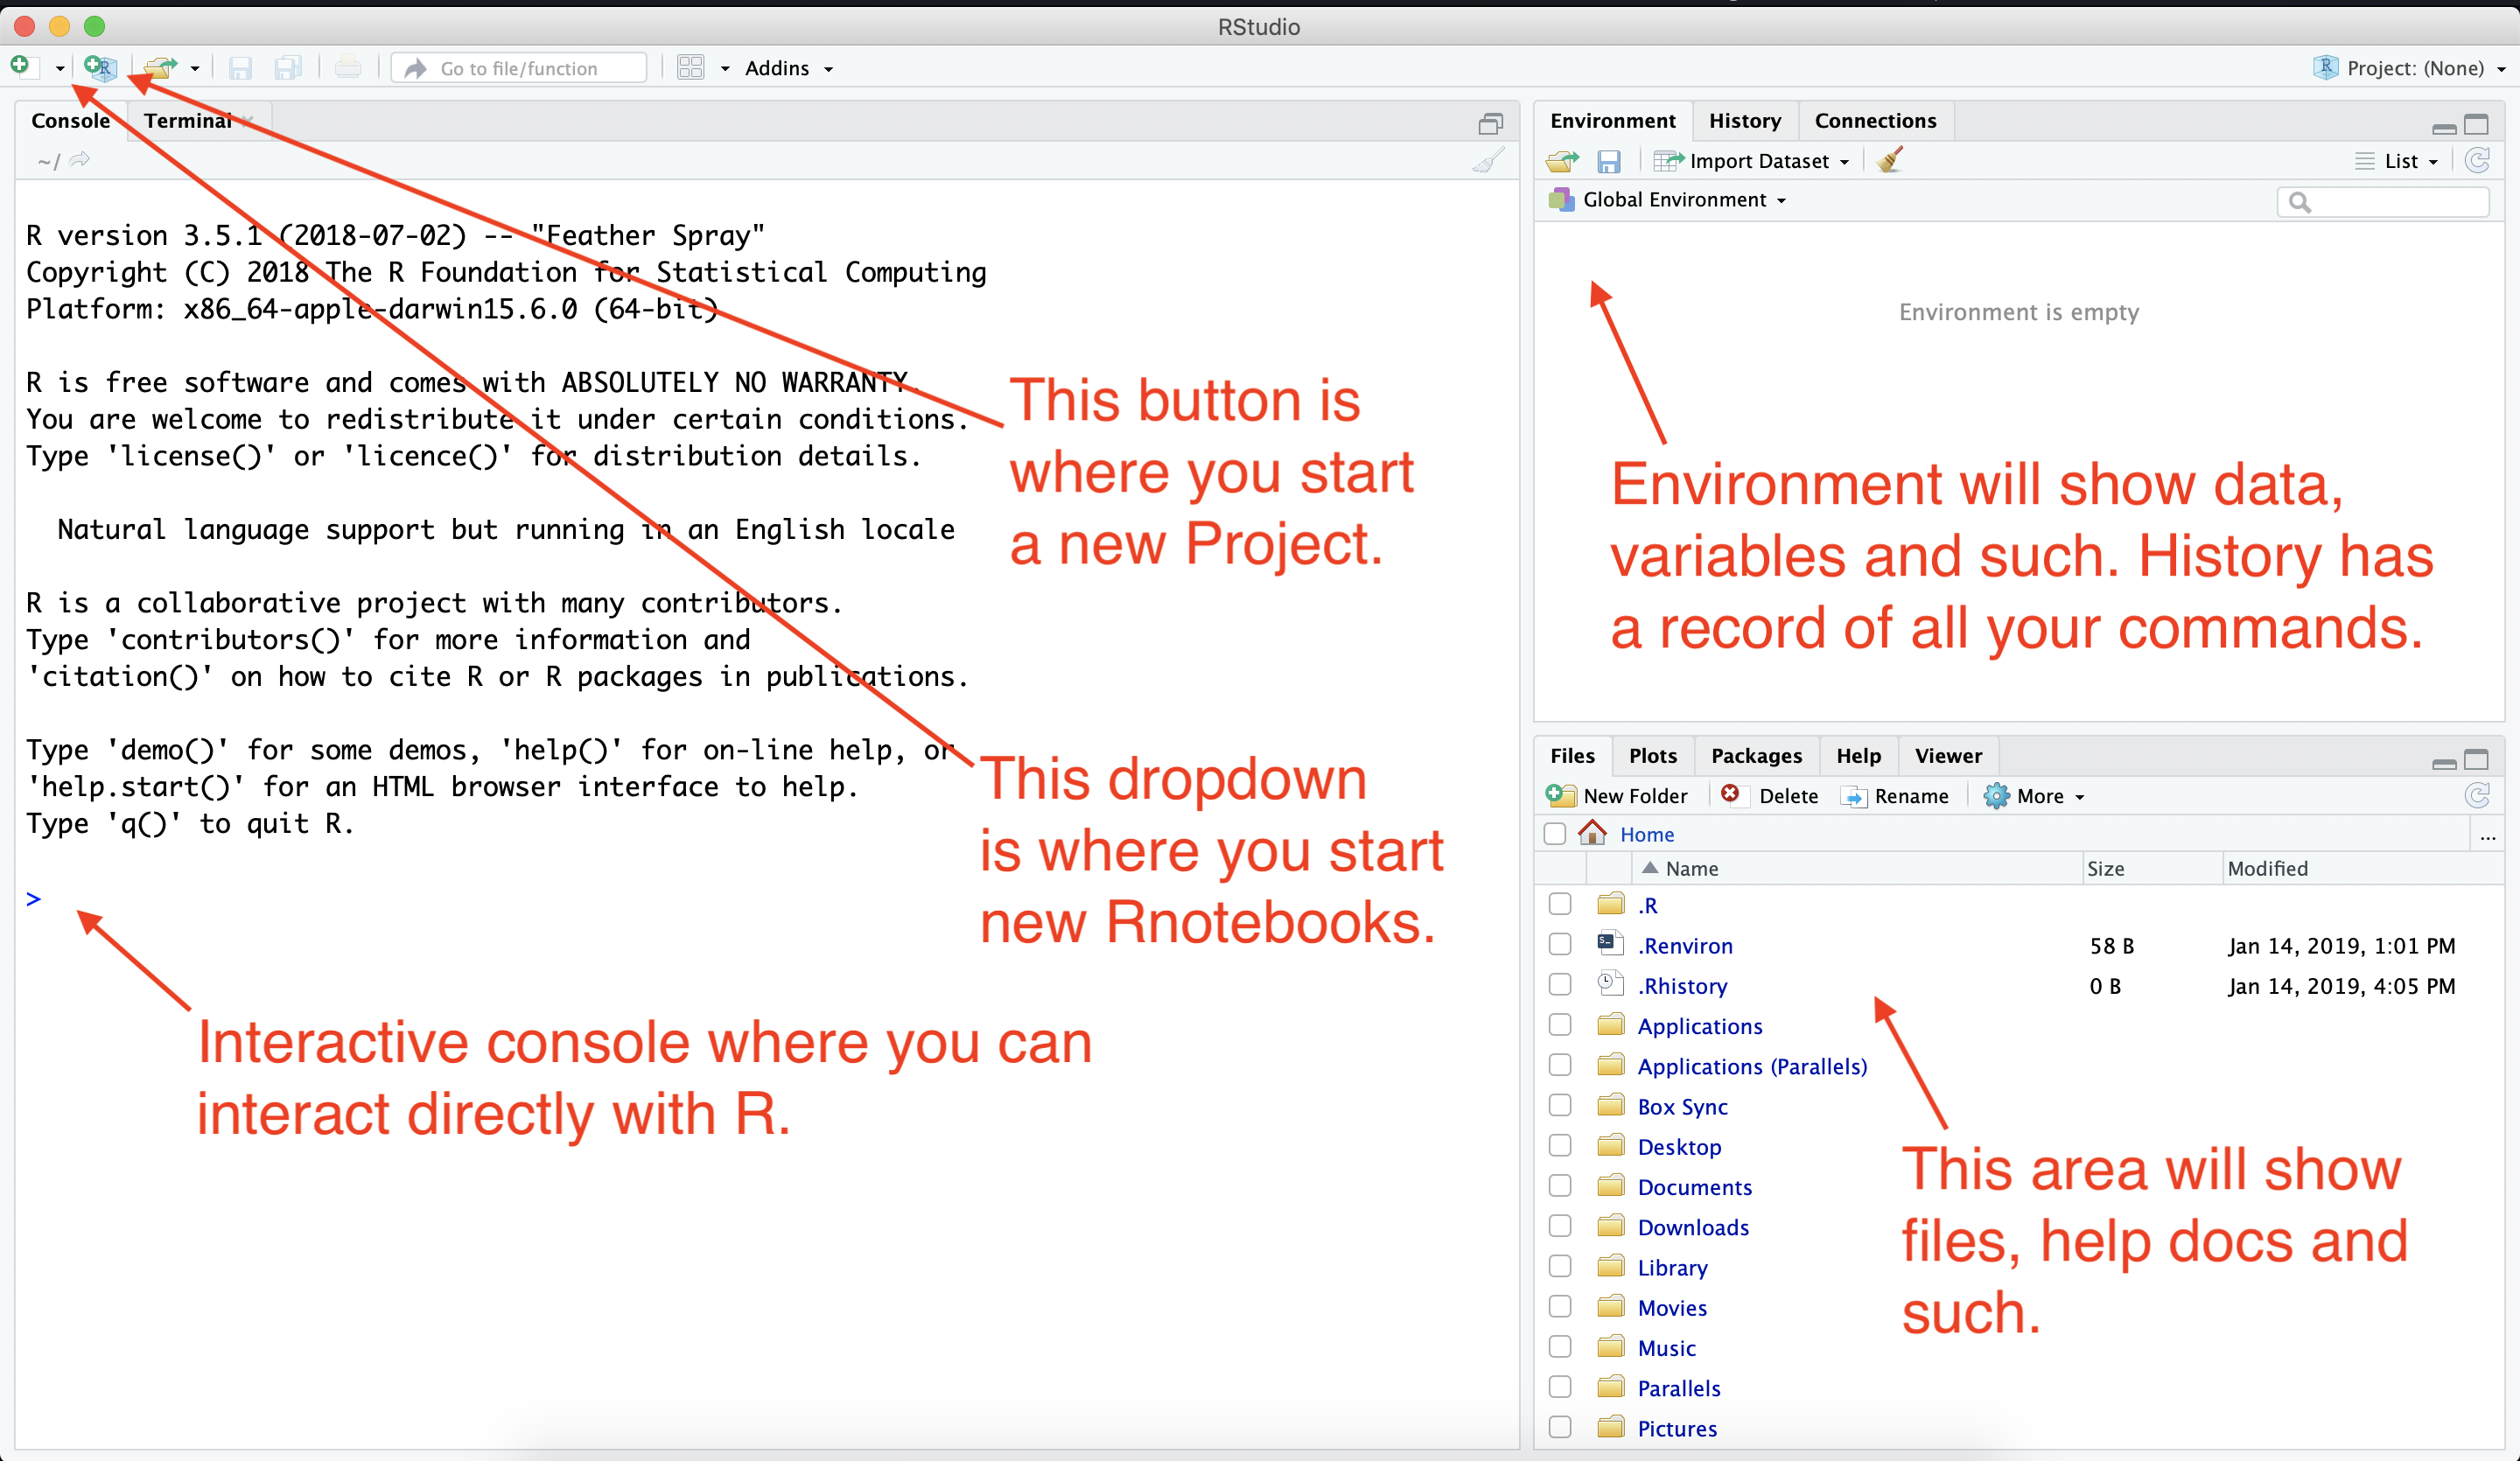
\includegraphics[width=0.5\linewidth]{_images/02-rstudio-start}

When you launch RStudio, you'll get a screen that looks like this:

\begin{figure}
\centering
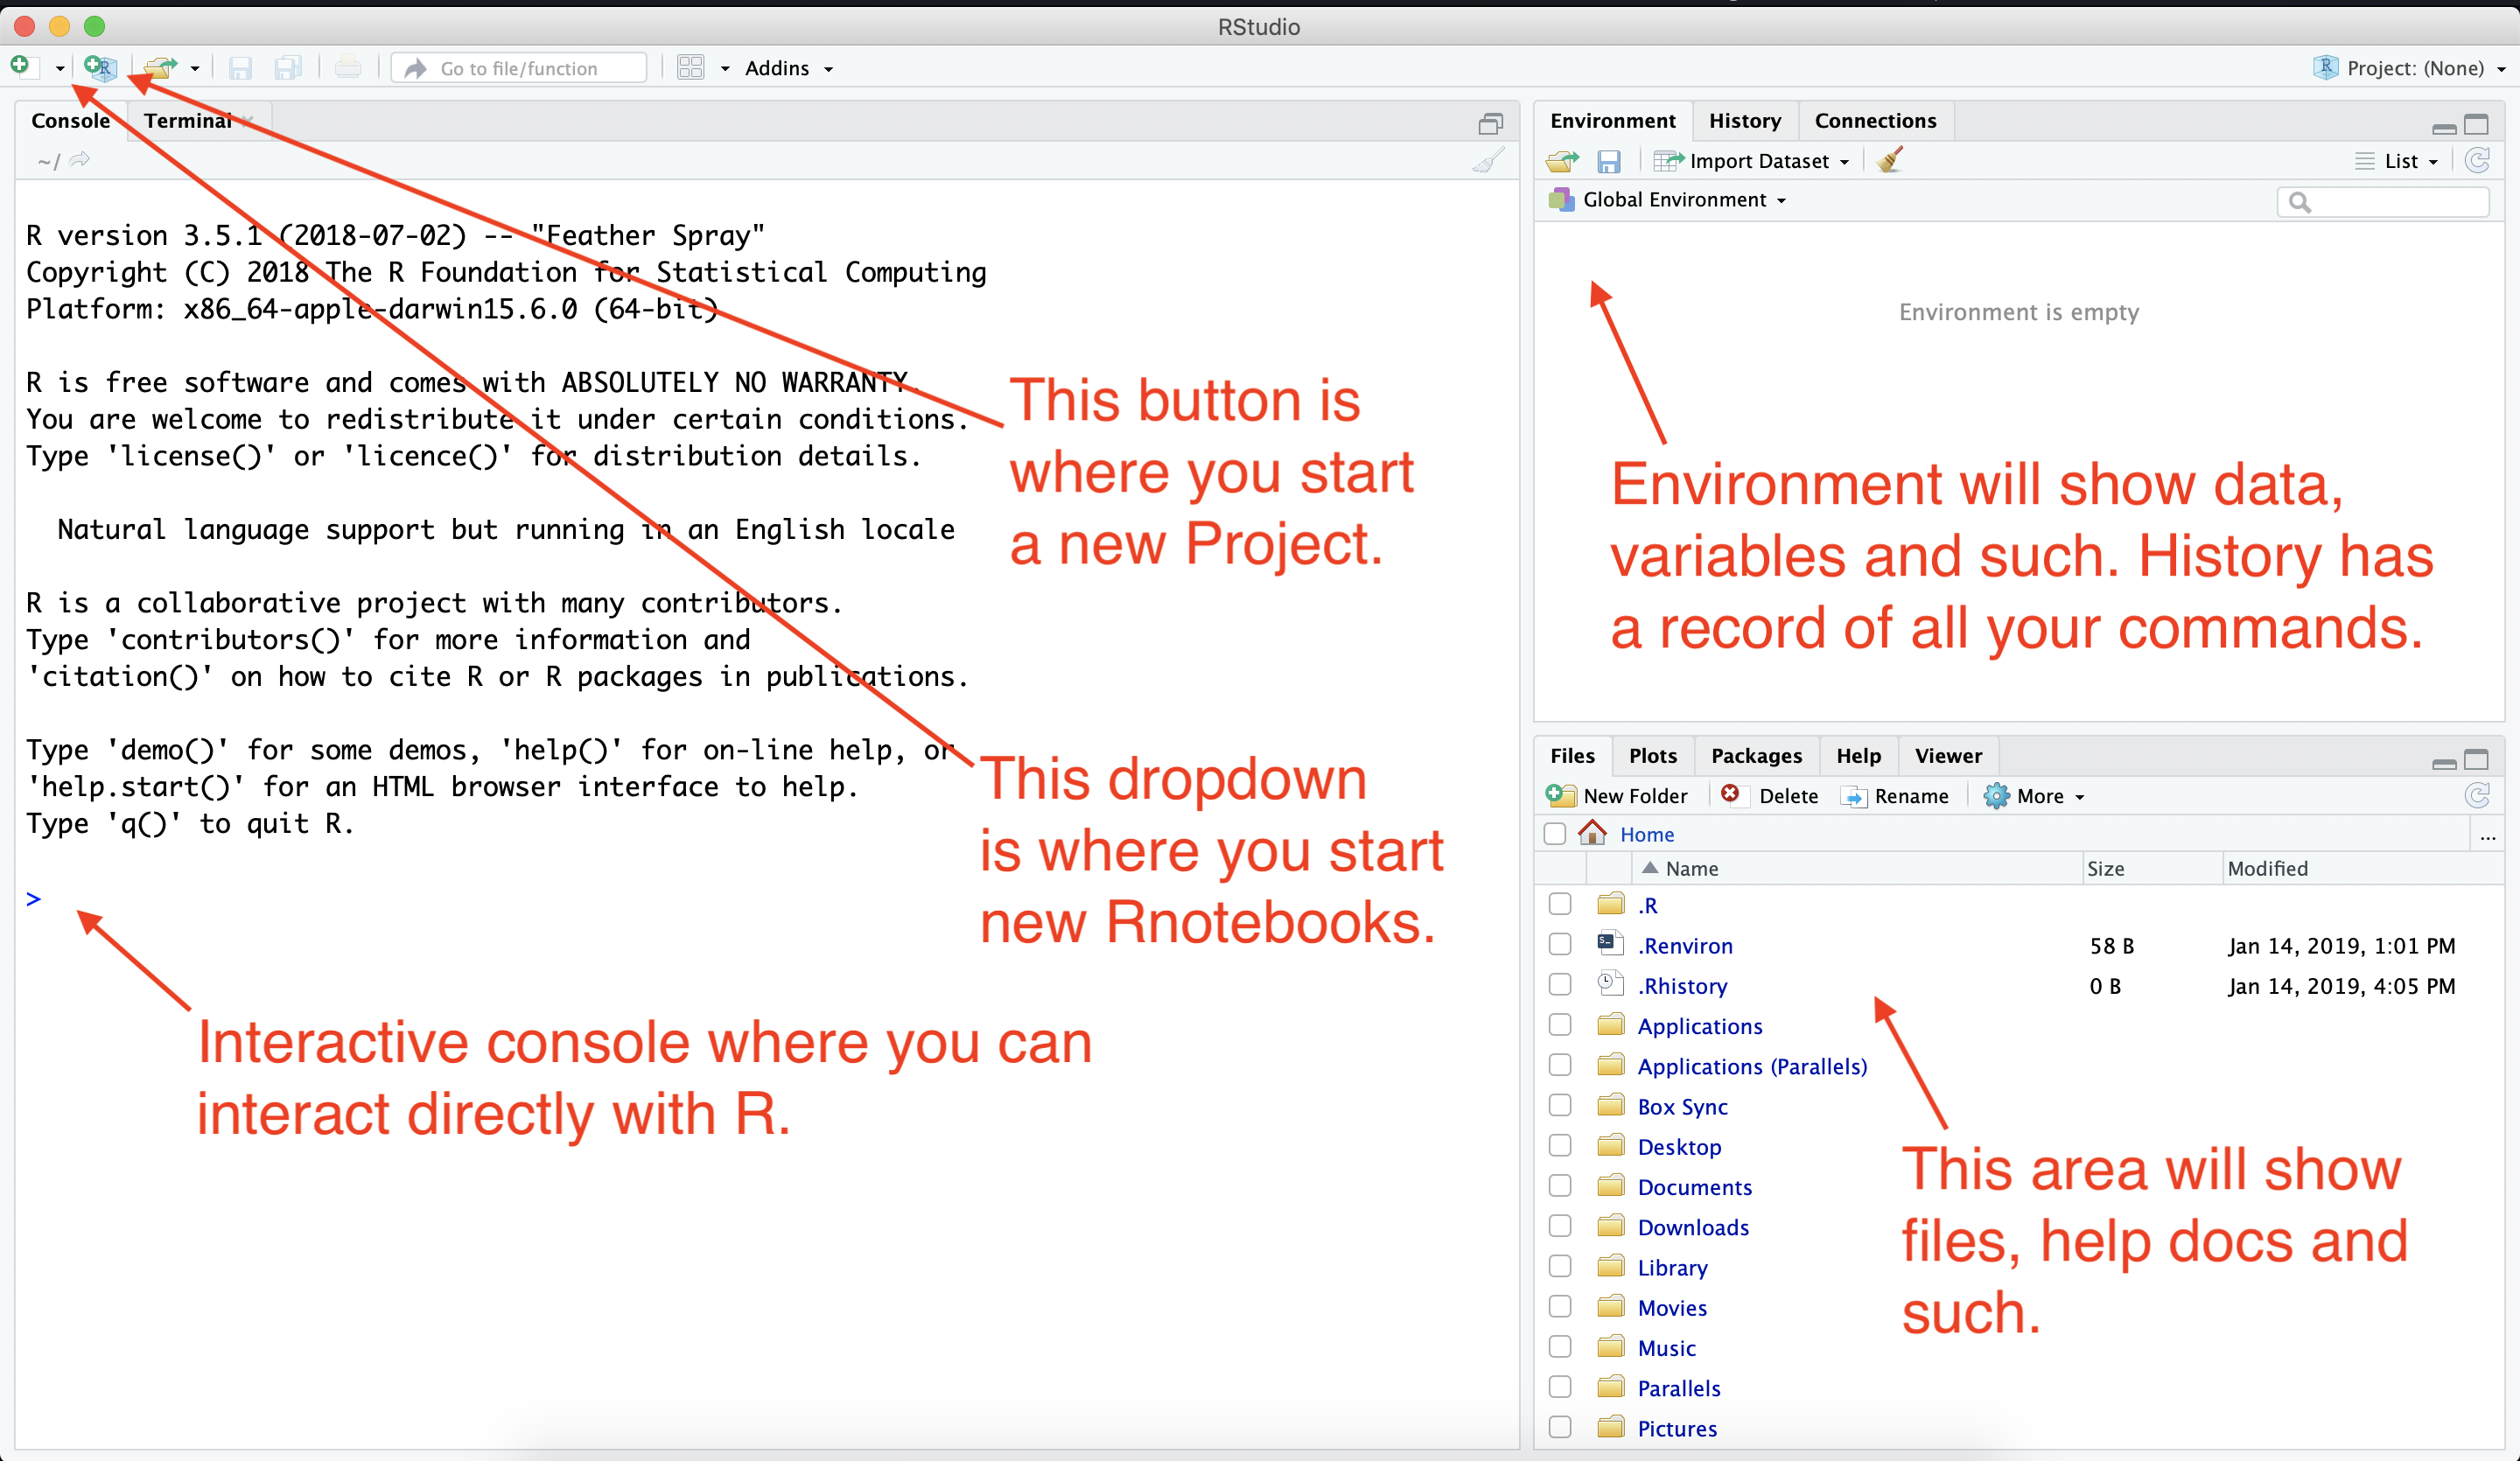
\includegraphics[width=6.25000in]{_images/02-rstudio-start.png}
\caption{Rstudio launch screen}
\end{figure}

\section{Starting a new Project}\label{starting-a-new-project}

When we work in RStudio, we will create ``Projects'' to hold all the
files related to one another. This sets the ``working directory'', which
is a sort of home base for the project.

\begin{itemize}
\tightlist
\item
  Click on the second button that has a green \texttt{+R} sign.
\item
  That brings up a box to create the project with several options. You
  want \textbf{New Directory} (unless you already have a Project
  directory, which you don't for this.)
\item
  For \textbf{Project Type}, choose \textbf{New Project}.
\item
  Next, for the \textbf{Directory name}, choose a new name for your
  project folder. For this project, use ``firstname-first-project'' but
  use YOUR firstname.
\end{itemize}

I want you to be anal about naming your folders. It's a good programming
habit.

\begin{itemize}
\tightlist
\item
  Use lowercase characters.
\item
  Don't use spaces. Use dashes.
\item
  For this class, start with your first name.
\end{itemize}

\begin{figure}
\centering
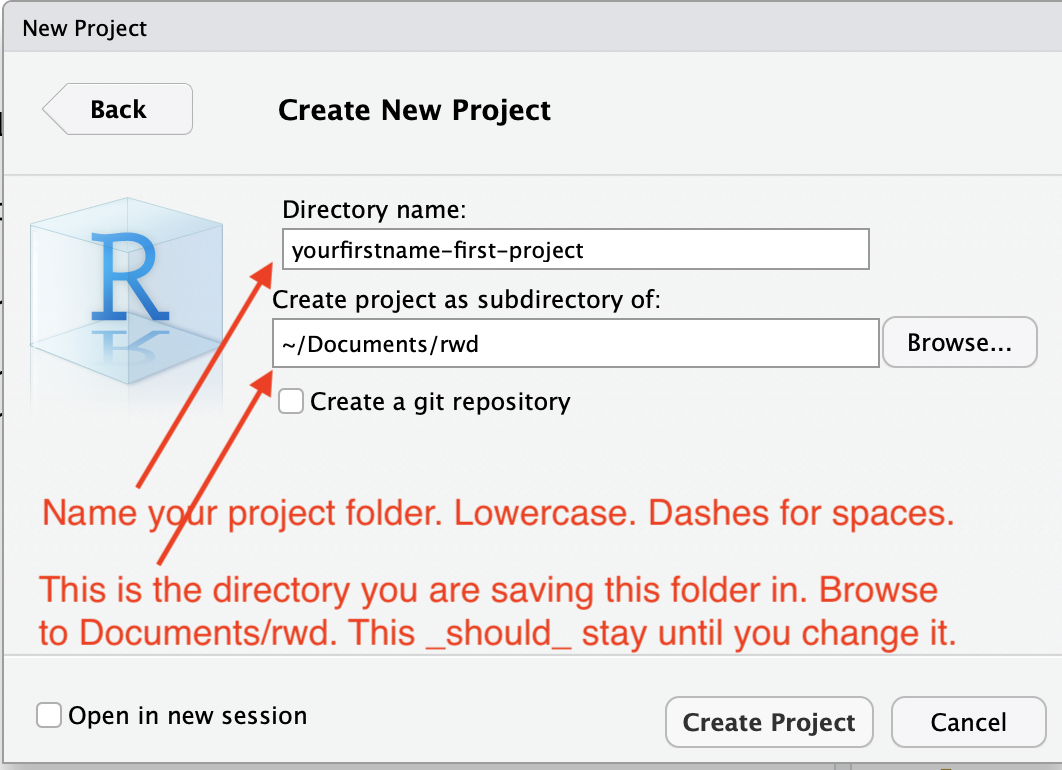
\includegraphics[width=4.16667in]{_images/02-rstudio-newproject.png}
\caption{Rstudio project name, directory}
\end{figure}

When you do this, your RStudio window will refresh and you'll see the
\texttt{yourfirstname-first-project.Rproj} file in your Files list.

\section{Using R Notebooks}\label{using-r-notebooks}

For this class, we will almost always use
\href{https://rmarkdown.rstudio.com/lesson-10.html}{R Notebooks}. This
format allows us to write text inbetween our blocks of code. The text is
written in a language called
\href{https://rmarkdown.rstudio.com/lesson-1.html}{R Markdown}. It
allows us to write text that gets turned into pretty HTML for our
reports. The R Markdown syntax is not hard. It is based on vanilla
Markdown, which is a common documentation syntax for programmers.

\subsection{Create your first
notebook}\label{create-your-first-notebook}

\begin{itemize}
\tightlist
\item
  Click on the button at the top-left of RStudio that has just the green
  \texttt{+} sign.
\item
  Choose the item \textbf{R Notebook}.
\end{itemize}

This will open a new file with some boilerplate R Markdown code.

\begin{itemize}
\tightlist
\item
  At the top between the \texttt{-\/-\/-} marks, is the
  \textbf{metadata}. This is written using YAML, and what is inside are
  commands for the R Notebook. Don't sweat the YAML syntax too much
  right now, as we won't be editing it often.
\item
  Next, you'll see a couple of paragraphs of text that describes how to
  use an R Notebooks. It is written in R Markdown, and has some inline
  links and bolding commands, which you will learn,
\item
  Then you will see an R code chunk that looks like the figure below.
\end{itemize}

\begin{figure}
\centering
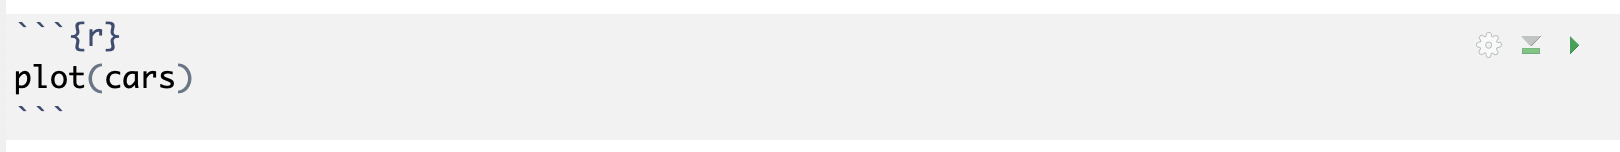
\includegraphics[width=6.25000in]{_images/02-rstudio-rcodechunk.png}
\caption{R code chunk}
\end{figure}

Let's take a closer look at this:

\begin{itemize}
\tightlist
\item
  The three backticks characters ( found at the top left on your
  keyboard) followed by the \texttt{\{r\}} indicate that this is a chunk
  of R code. The last three backticks say the code chunk is over.
\item
  The \texttt{\{r\}} bit can have some parameters added to it. We'll get
  into that later.
\item
  The line \texttt{plot(cars)} is R programming code. We'll see what
  those commands do in a bit.
\item
  The green right-arrow to the far right is a play button to run the
  code that is inside the chunk.
\item
  The green down-arrow and bar to the left of that runs all the code in
  the Notebook up to that point.
\end{itemize}

\subsection{Save the .Rmd file}\label{save-the-.rmd-file}

\begin{itemize}
\tightlist
\item
  Do command-s or hit the floppy disk icon to save the file.
\item
  It will ask you what you want to name this file. Call it
  \texttt{01-first-file.Rmd}.
\end{itemize}

When you do this, you may see another new file created in your Files
directory. It's the pretty version of the notebook which we'll see in a
minute.

In the metadata portion of the file, give your notebook a better title.

\begin{itemize}
\tightlist
\item
  Replace ``R Notebook'' in the \texttt{title:\ "R\ Notebook"} code to
  be ``Christian's first notebook'', but use your name.
\end{itemize}

\subsection{Run the notebook}\label{run-the-notebook}

There is only one chunk to run in this notebook, so:

\begin{itemize}
\tightlist
\item
  Click on the green right-arrow to run the code.
\end{itemize}

You should get something like this:

\begin{figure}
\centering
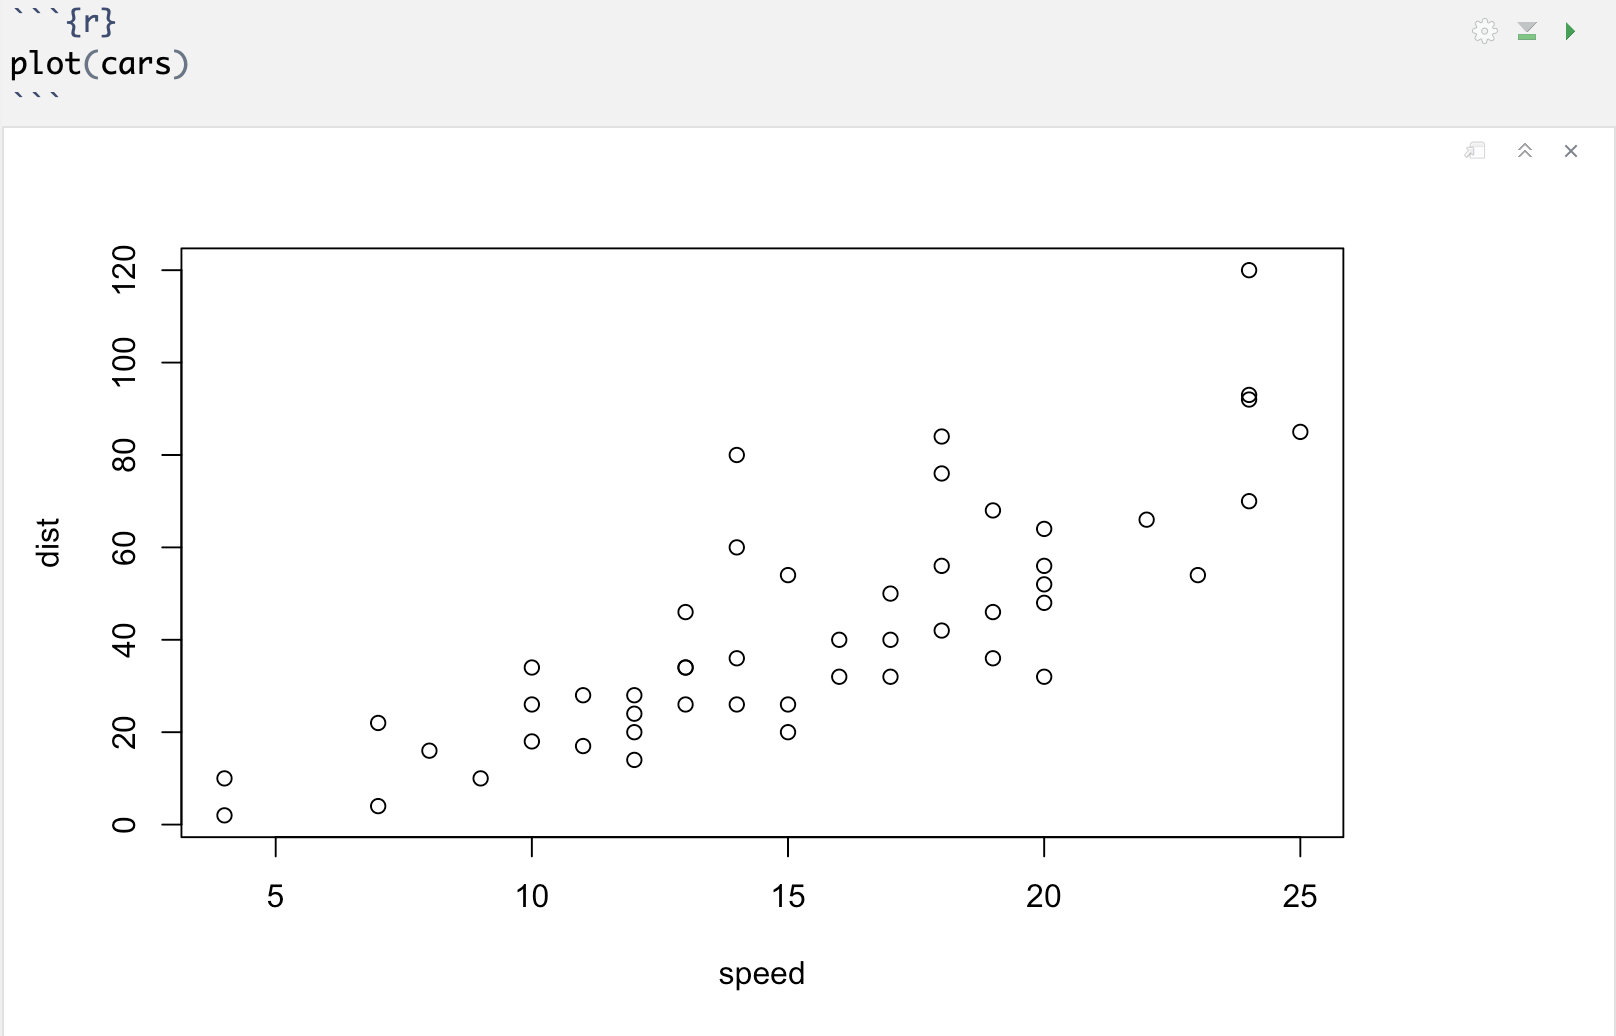
\includegraphics[width=6.25000in]{_images/02-rstudio-defaultplot.png}
\caption{Cars plot}
\end{figure}

What you've done here is create a plot chart of a piece of sample data
that is already inside R. (FWIW, It is the speed of cars and the
distances taken to stop. Note that the data were recorded in the 1920s.)

But that wasn't a whole lot of code to see there is a relationship with
speed vs stopping distince, eh?

\subsection{Adding new code chunks}\label{adding-new-code-chunks}

The text after the chart describes how you an insert a new code chunk.
After that text, I'd like you to do that.

\begin{itemize}
\tightlist
\item
  After the text that describes how to add code, but before the next bit
  of text, add a new code junk with \emph{Cmd+Option+I}.
\item
  Your cursor will be inserted into the middle of the chunk. Type in
  this code:
\end{itemize}

\begin{verbatim}
# min age to date
age = 52
(age / 2) + 7
\end{verbatim}

\begin{itemize}
\tightlist
\item
  Change for ``52'' to your real age.
\item
  With your cursor somewhere in the code block, use the key command
  \emph{Cmd+Shift+Return}, which is the key command two run an ENTIRE
  chunk.
\item
  NOTE: To run an individual line, use \emph{Cmd+Return} while on that
  line.
\end{itemize}

Congratualtions! The answer given at the bottom of that code chunk is
the
\href{https://www.psychologytoday.com/us/blog/meet-catch-and-keep/201405/who-is-too-young-or-too-old-you-date}{socially-acceptable
minimum age of anyone you should date}.

Throwing aside whether the formula is sound, let's break down the code.

\begin{itemize}
\tightlist
\item
  \texttt{\#\ min\ age\ to\ date} is a comment. It's a way to explain
  what is happening in the code without being considered part of the
  code.
\item
  \texttt{age\ =\ 51} is assigning a number (\texttt{52}) to a variable
  name (\texttt{age}).
\item
  \texttt{(age\ /\ 2)\ +\ 7} takes the value of \texttt{age} and divides
  that by \texttt{2}, then adds \texttt{7}.
\end{itemize}

Now you can play with the age variable assignment to test out different
ages.

\subsection{Practice adding code
chunks}\label{practice-adding-code-chunks}

Now, on your own, add a similar code chunck that calculates the maximum
age of someone you should date, but using the formula
\texttt{(age\ -\ 7)\ *\ 2}.

\subsection{Preview the report}\label{preview-the-report}

The rest of the boilerplate text here describes how you can \emph{Knit}
or \emph{Preview} a notebook. Let's do that now.

\begin{itemize}
\tightlist
\item
  Press \emph{Cmd+Shift+K} to open a Preview.
\end{itemize}

This will open a new window and how you the ``pretty'' notebook that we
are building. It's really an HTML file that was create by RStudio. (You
can also open this in a web browser).

Preview is a little different than \emph{Knit}, which runs all the code,
then creates the new knitted document.

\subsection{The toolbar}\label{the-toolbar}

Last thing to describe before we turn this in is the toolbar that runs
across the top of the R Notebook file window.

\begin{figure}
\centering
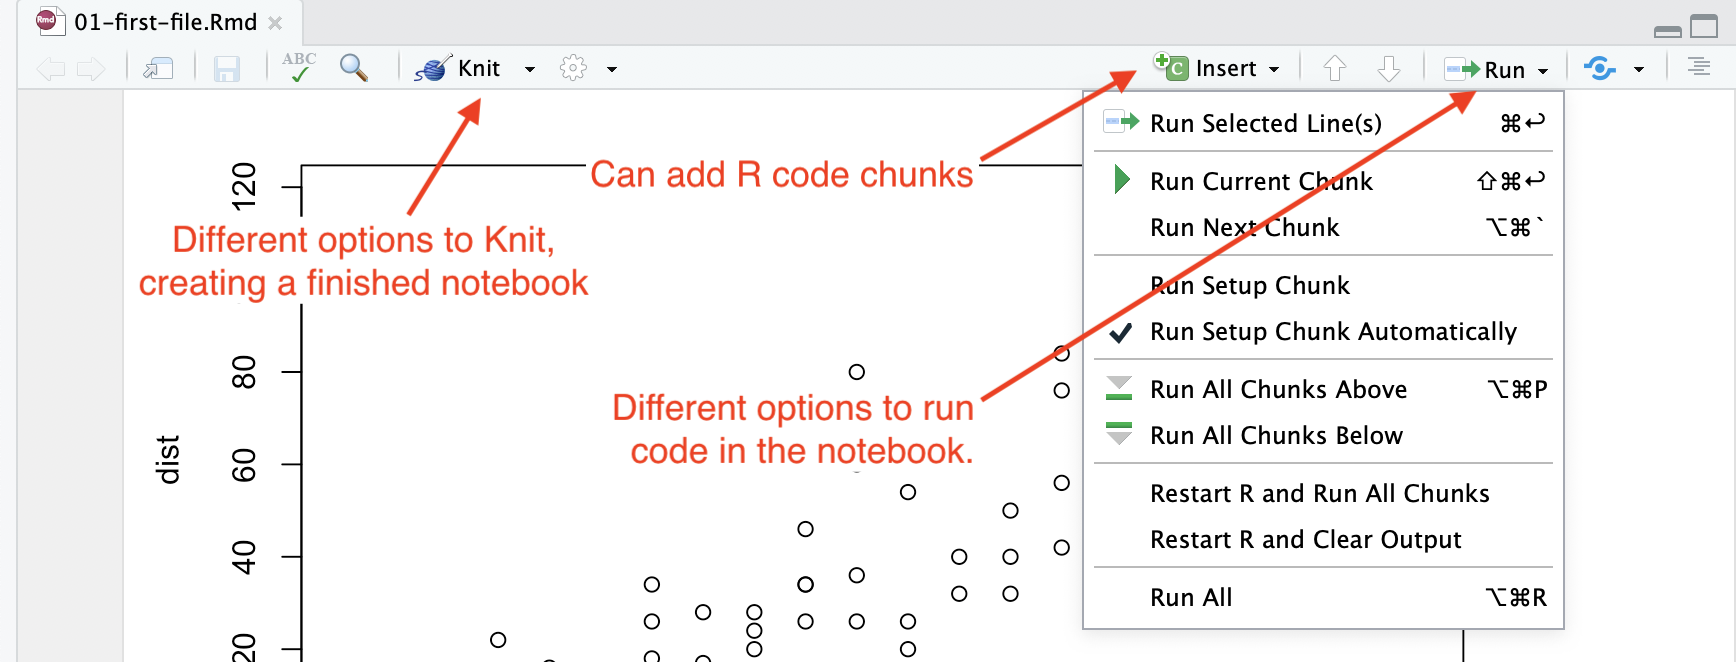
\includegraphics[width=6.25000in]{_images/02-rstudio-toolbar.png}
\caption{R Notebook toolbar}
\end{figure}

\subsection{Knit the final workbook}\label{knit-the-final-workbook}

\begin{itemize}
\tightlist
\item
  Save your File with \emph{Cmd+S}.
\item
  Use the \textbf{Knit} button to choose \textbf{Knit to HTML}.
\end{itemize}

\section{Turning in our projects}\label{turning-in-our-projects}

So now if you look in your Files pane, you'll see you have four files in
our project.

\begin{figure}
\centering
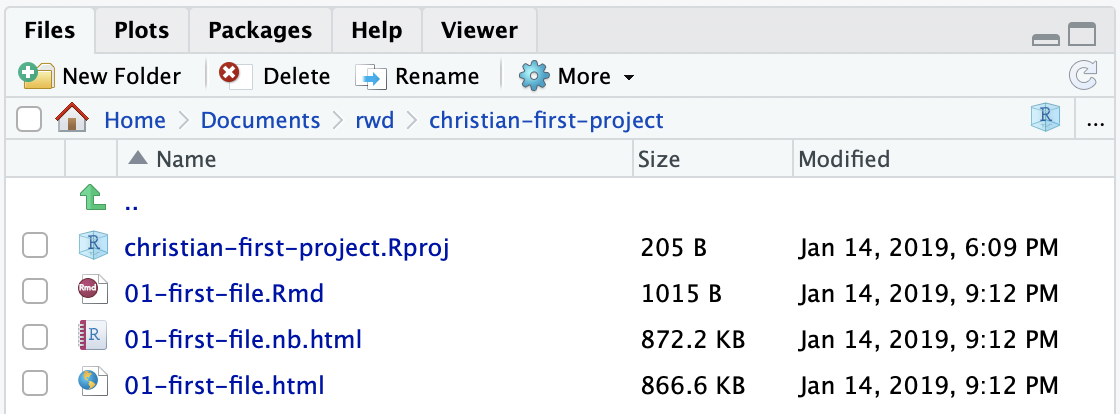
\includegraphics[width=5.20833in]{_images/02-rstudio-files.png}
\caption{Files list}
\end{figure}

Now we have to zip these all up into a single file that you can turn
into Canvas. (Note the only one you actually edit is the \texttt{.Rmd}
file.)

\begin{itemize}
\tightlist
\item
  In your computer's finder, open the \texttt{Documents/rwd} folder.
\item
  Follow the directions for your operating system linked below to create
  a compressed version of your \texttt{yourname-final-project} folder.
\item
  \href{http://www.macinstruct.com/node/159}{Compress files on a Mac}.
\item
  \href{https://www.laptopmag.com/articles/how-to-zip-files-windows-10}{Compress
  flies on Windows}.
\item
  Upload the resulting \texttt{.zip} file to the assignment for this
  week in Canvas.
\end{itemize}

Here is what the compression steps looks like on a Mac:

\begin{Shaded}
\begin{Highlighting}[]
\CommentTok{# ![Compress file: Mac](_images/02-rstudio-compress.gif)\{width=400px\}}
\end{Highlighting}
\end{Shaded}

If you find you make changes to your R files after you've zipped your
folder, you'll need to delete the \texttt{zip} file and do it again.

\chapter{Importing data}\label{import}

Lesson about imports, data frames, embedded data.

This
\href{https://www.datacamp.com/community/tutorials/r-data-import-tutorial\#spss}{DataCamp}
tutorial may come in handy.

\chapter{Data manipulation}\label{manipulation}

About using dpylr to filter, sort and manipulate data.

\chapter{Data types}\label{datatypes}

About dealing with dates and other data types.

\chapter{Aggregation}\label{aggregation}

About aggregation, creating new columns, etc.

\chapter{Tidy data}\label{tidy}

About shaping data with tidyr.

\chapter{Graphics}\label{graphics}

This is an \href{http://rmarkdown.rstudio.com}{R Markdown} Notebook.
When you execute code within the notebook, the results appear beneath
the code.

Try executing this chunk by clicking the \emph{Run} button within the
chunk or by placing your cursor inside it and pressing
\emph{Cmd+Shift+Enter}.

\begin{Shaded}
\begin{Highlighting}[]
\KeywordTok{plot}\NormalTok{(cars)}
\end{Highlighting}
\end{Shaded}

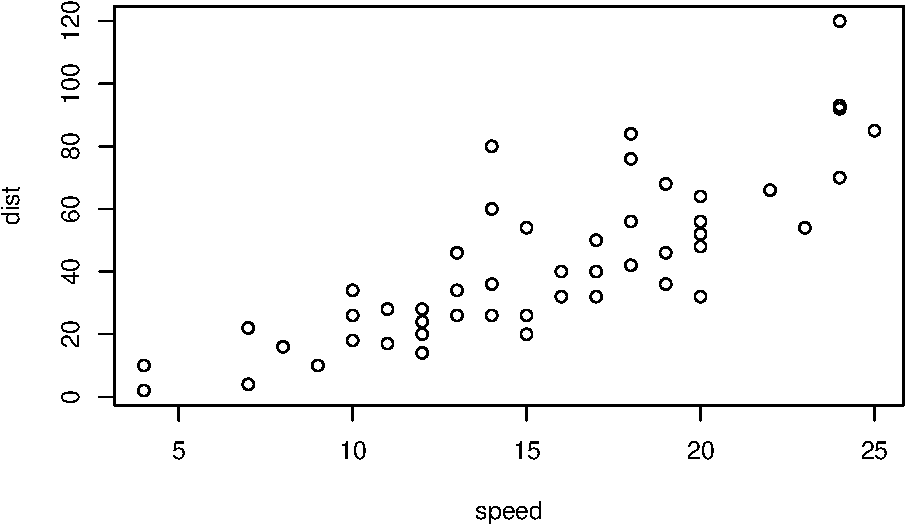
\includegraphics{08-graphics_files/figure-latex/unnamed-chunk-1-1.pdf}

Add a new chunk by clicking the \emph{Insert Chunk} button on the
toolbar or by pressing \emph{Cmd+Option+I}.

When you save the notebook, an HTML file containing the code and output
will be saved alongside it (click the \emph{Preview} button or press
\emph{Cmd+Shift+K} to preview the HTML file).

The preview shows you a rendered HTML copy of the contents of the
editor. Consequently, unlike \emph{Knit}, \emph{Preview} does not run
any R code chunks. Instead, the output of the chunk when it was last run
in the editor is displayed.

\chapter{Census}\label{census}

A mini project using census data.

\section{Resources}\label{resources}

\begin{itemize}
\tightlist
\item
  \href{https://rconsortium.github.io/censusguide/}{Census guide}
\item
  \href{https://www.computerworld.com/article/3120415/data-analytics/how-to-download-new-census-data-with-r.html}{Sharon
  Machlis guide}
\item
  \href{https://cran.r-project.org/web/packages/acs/README.html}{acs
  package}
\item
  \citet{hrecht} if News Nerdery is author of the {[}censusapi
  package{]}
\item
  \href{https://github.com/baltimore-sun-data/census-data-analysis-2018}{Baltimore
  Sun example}. ``sometimes i prefer the output of one over the other
  \texttt{censusapi} vs \texttt{tidycensus}, which is why i alternate. i
  also for some reason didn't realize i could have used the R packages
  to download the SAIPE (poverty stats) data; in the repo I just
  downloaded the file from the site''.
\item
  \href{http://api.census.gov/data/key_signup.html}{API key signup}
\end{itemize}

\chapter{Joins and merges}\label{joins}

About joins, merges and the like.

\chapter{Data packages}\label{data}

About various data packages and such.

\chapter{Maps}\label{maps}

About making maps.

\chapter*{References}\label{references}
\addcontentsline{toc}{chapter}{References}

Figures and tables with captions will be placed in \texttt{figure} and
\texttt{table} environments, respectively.

\begin{Shaded}
\begin{Highlighting}[]
\KeywordTok{par}\NormalTok{(}\DataTypeTok{mar =} \KeywordTok{c}\NormalTok{(}\DecValTok{4}\NormalTok{, }\DecValTok{4}\NormalTok{, .}\DecValTok{1}\NormalTok{, .}\DecValTok{1}\NormalTok{))}
\KeywordTok{plot}\NormalTok{(pressure, }\DataTypeTok{type =} \StringTok{'b'}\NormalTok{, }\DataTypeTok{pch =} \DecValTok{19}\NormalTok{)}
\end{Highlighting}
\end{Shaded}

\begin{figure}

{\centering 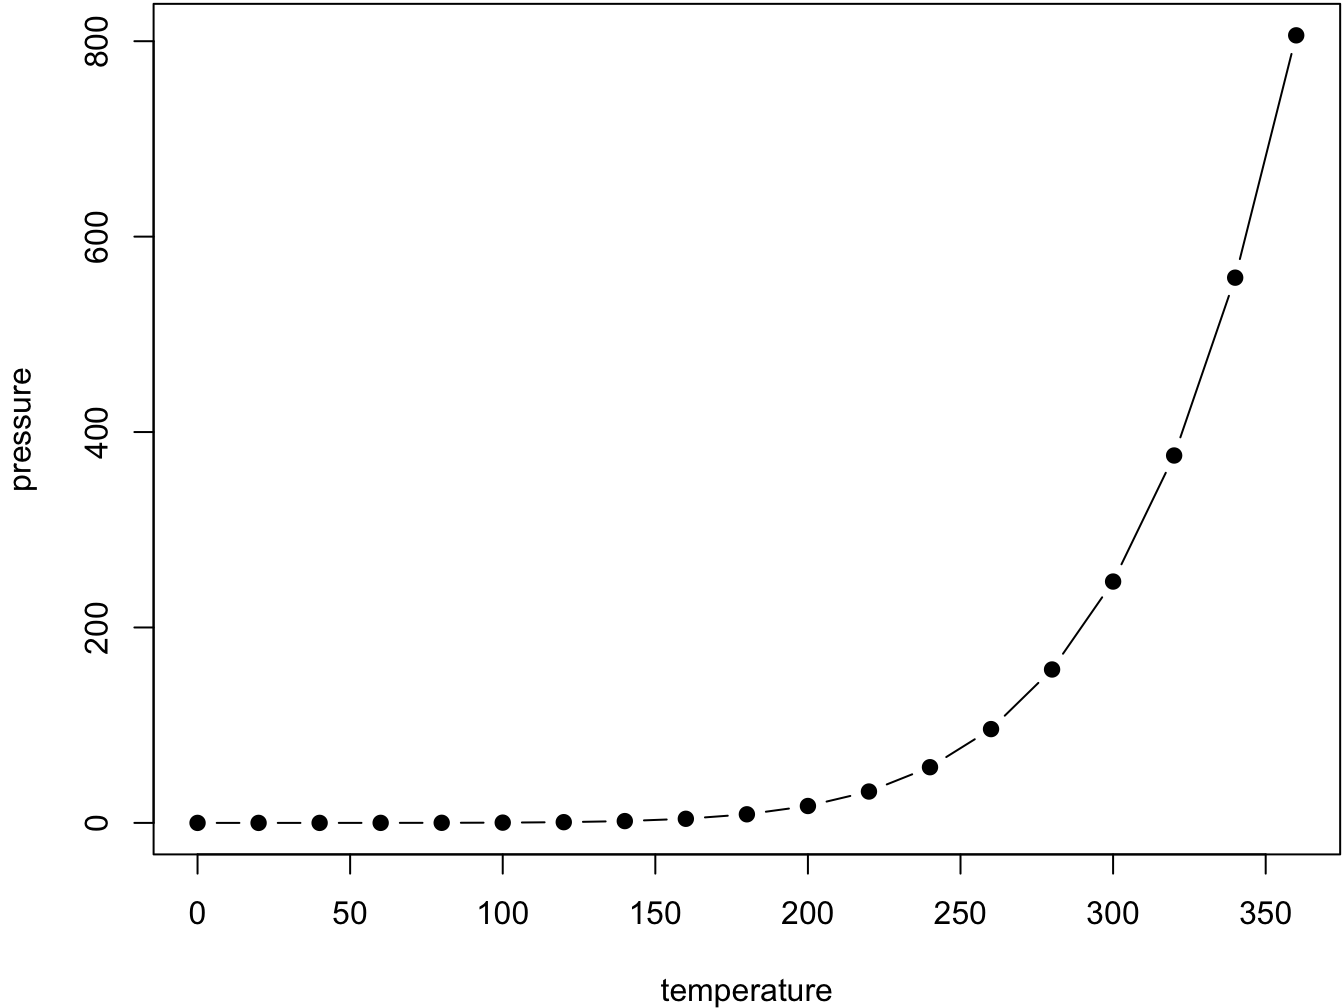
\includegraphics[width=0.8\linewidth]{99-references_files/figure-latex/nice-fig-1} 

}

\caption{Here is a nice figure!}\label{fig:nice-fig}
\end{figure}

Reference a figure by its code chunk label with the \texttt{fig:}
prefix, e.g., see Figure \ref{fig:nice-fig}. Similarly, you can
reference tables generated from \texttt{knitr::kable()}, e.g., see Table
\ref{tab:nice-tab}.

\begin{Shaded}
\begin{Highlighting}[]
\NormalTok{knitr}\OperatorTok{::}\KeywordTok{kable}\NormalTok{(}
  \KeywordTok{head}\NormalTok{(iris, }\DecValTok{20}\NormalTok{), }\DataTypeTok{caption =} \StringTok{'Here is a nice table!'}\NormalTok{,}
  \DataTypeTok{booktabs =} \OtherTok{TRUE}
\NormalTok{)}
\end{Highlighting}
\end{Shaded}

\begin{table}

\caption{\label{tab:nice-tab}Here is a nice table!}
\centering
\begin{tabular}[t]{rrrrl}
\toprule
Sepal.Length & Sepal.Width & Petal.Length & Petal.Width & Species\\
\midrule
5.1 & 3.5 & 1.4 & 0.2 & setosa\\
4.9 & 3.0 & 1.4 & 0.2 & setosa\\
4.7 & 3.2 & 1.3 & 0.2 & setosa\\
4.6 & 3.1 & 1.5 & 0.2 & setosa\\
5.0 & 3.6 & 1.4 & 0.2 & setosa\\
\addlinespace
5.4 & 3.9 & 1.7 & 0.4 & setosa\\
4.6 & 3.4 & 1.4 & 0.3 & setosa\\
5.0 & 3.4 & 1.5 & 0.2 & setosa\\
4.4 & 2.9 & 1.4 & 0.2 & setosa\\
4.9 & 3.1 & 1.5 & 0.1 & setosa\\
\addlinespace
5.4 & 3.7 & 1.5 & 0.2 & setosa\\
4.8 & 3.4 & 1.6 & 0.2 & setosa\\
4.8 & 3.0 & 1.4 & 0.1 & setosa\\
4.3 & 3.0 & 1.1 & 0.1 & setosa\\
5.8 & 4.0 & 1.2 & 0.2 & setosa\\
\addlinespace
5.7 & 4.4 & 1.5 & 0.4 & setosa\\
5.4 & 3.9 & 1.3 & 0.4 & setosa\\
5.1 & 3.5 & 1.4 & 0.3 & setosa\\
5.7 & 3.8 & 1.7 & 0.3 & setosa\\
5.1 & 3.8 & 1.5 & 0.3 & setosa\\
\bottomrule
\end{tabular}
\end{table}

You can write citations, too. For example, we are using the
\textbf{bookdown} package \citep{R-bookdown} in this sample book, which
was built on top of R Markdown and \textbf{knitr} \citep{xie2015}.

\bibliography{book.bib,packages.bib}


\end{document}
